\documentclass[11pt]{article}
\usepackage{amsmath}
\usepackage{amssymb}
\usepackage{amsthm}
\usepackage{amscd}
\usepackage{amsfonts}
\usepackage{graphicx}%
\usepackage{fancyhdr}
\usepackage{color}
\usepackage{cite}

\usepackage{longtable}

%\usepackage[T1]{fontenc}
\usepackage[utf8]{inputenc}
\usepackage{authblk}
\usepackage{physics}
\usepackage{float}
\usepackage{caption}
\usepackage{subcaption}
\newcommand{\expv}[1]{\ensuremath{\mathbb{E}[ #1]}}
\newcommand{\xs}[2]{\ensuremath{\Sigma_{#1}^{(#2)}}}
\newcommand{\intO}{\ensuremath{\int\limits_{4\pi}}}
\newcommand{\intnp}{\ensuremath{\int\limits_{-1}^1}}
\newcommand{\intab}[1]{\ensuremath{\int\limits_{a_{#1}}^{b_#1}}}
\newcommand{\intz}{\ensuremath{\int\limits_0^1}}
\newcommand{\intf}{\ensuremath{\int\limits_{-\infty}^\infty}}
\newcommand{\intzf}{\ensuremath{\int\limits_{0}^\infty}}
\newcommand{\LargerCdot}{\raisebox{-0.25ex}{\scalebox{1.2}{$\cdot$}}}

\textwidth6.6in
\textheight9in


\setlength{\topmargin}{0.3in} \addtolength{\topmargin}{-\headheight}
\addtolength{\topmargin}{-\headsep}

\setlength{\oddsidemargin}{0in}

\oddsidemargin  0.0in \evensidemargin 0.0in \parindent0em

%\pagestyle{fancy}\lhead{MATH 579 (UQ for PDEs)} \rhead{02/24/2014}
%\chead{Project Proposal} \lfoot{} \rfoot{\bf \thepage} \cfoot{}


\begin{document}

\title{Failure Case for the Smolyak Sparse Quadrature for gPC Expansion}

\author[]{Paul Talbot\thanks{talbotp@unm.edu}}
\date{}
\renewcommand\Authands{ and }
\maketitle
\section{Introduction}
Let $(\Omega,\mathcal{F},\rho)$ be a complete $N$-variate probability space.
We consider the algorithms for expanding a quantity of interest $u(Y)$ as a function of uncertain independent
input parameters $Y = (y_1,\cdots,y_n,\cdots,y_N)$ in a generalized polynomial chaos expansion using
orthonormal Gaussian polynomials $\phi_i^{(n)}(y_n)$.  These Gaussian polynomials are orthonormal with respect
to their corresponding individual monovariate probability space $(\Omega_n,\mathcal{F}_n,\rho_n)$.  The
expansion is given by
\begin{equation}\label{eq:gpc}
  u(Y)\approx \tilde u(Y) = \sum_{k\in\Lambda} c_k \Phi_k(Y),
\end{equation}
where $k$ is a multivariate index, $\Lambda$ is a set of $N$-variate indices corresponding to polynomial
orders, and $\Phi_k$ are a set of orthonormal multidimensional polynomials given by
\begin{equation}
  \Phi_k(Y) = \prod_{n=1}^N \phi_{k_n}(y_n).
\end{equation}
We assume $\Lambda$ can be constructed adaptively.  The admissability condition for new indices $k$ into
$\Lambda$ is
\begin{equation}
  k-e_j \in \Lambda \forall 1\leq j\leq N\,
\end{equation}
where $e_j$ is a unit vector in the direction of $j$.

The scalar coefficients $c_k$ in Eq. \ref{eq:gpc} can be obtained via the orthonormality of $\Phi_k$ as
\begin{equation}\label{eq:coeffs}
  c_k = \int_\Omega \rho(Y) u(Y) \Phi_k(Y) dY \equiv \mathcal{I}\big(u\cdot\Phi_k\big).
\end{equation}
We approximate the integral using Smolyak-like sparse quadrature. Using the notation for a single-dimension
quadrature operation
\begin{equation}
  \int \rho(x)f(x)dx = \mathcal{I}(f) \approx \sum_{\ell=1}^L w_\ell f(x_\ell) \equiv q^{L}(f),
\end{equation}
the sparse quadrature is given by
\begin{equation}
  \mathcal{I}\big(u\cdot\Phi\big)\approx\mathcal{S}[u\cdot\Phi]\equiv \sum_{\hat k\in\Lambda} s_{\hat k} \bigotimes_{n=1}^N
  q^{L_n}\big(u(Y)\Phi_k(Y)\big).
\end{equation}
The quadrature coefficient $s_{\hat k}$ is given by
\begin{equation}
  s_{\hat k} = \sum_{j\in\{0,1\}^N,i+j\in\Lambda} (-1)^{|j|_1}, \hspace{10pt} |j|_1 = \sum_{n=1}^N j_n. 
\end{equation}

We present here a case with the convergence on analytic solutions for review.

\section{Case}
For demonstration, we consider a Gaussian peak from Genz (1984) with the following form:
\begin{equation}
  u(Y) = \exp[-\sum_{n=1}^N a_n^2(y_n-u_n)^2],
\end{equation}
with $Y = (y_1,\cdots,y_N)$ and all $y_n$ independently uniformly distributed from 0 to 1.  In this case, we use
orthonormalized Legendre polynomials for the expansion polynomials $\phi$.  While the scaling and location
factors $a_n$ and $u_n$ are arbitrary, we use $a_n = 5$ and $u_n = 1/2$ for all $1\leq n\leq N$.  For this
demonstration, we consider the two-dimensional input case ($N=2$).

\section{Taylor Analysis}
First, we consider the Taylor development of the function in question.  Since the location and scale are not
relevant to the general polynomial representation, we consider $a_n=1$ and $u_n=0$.  For the
single-dimensional case,
\begin{equation}
  u(y) = \exp[-y^2].
\end{equation}
The Taylor series expansion about $x=0$ for this is
\begin{equation}
  \exp[-y^2] = 1 - y^2 + \frac{y^4}{2!} - \frac{y^6}{3!} + \frac{y^8}{4!} -\cdots
\end{equation}
which contains all even-powered monomials in $x$ with decreasing amplitude as order increases.  The
two-dimension case then includes a tensor product of all even-valued polynomials for both $y_1$ and $y_2$.
Constructing a table of coefficient values, the first several terms in the combined Taylor development is
\begin{table}[H]
  \centering
  \caption{Taylor Development Polynomial Coefficients}
  \label{tab:taylor}
  \begin{tabular}{c|c c c c}
    3 & -1/6 &  1/6 & -1/12 &  1/36 \\
    2 &  1/2 & -1/2 &  1/4  & -1/12 \\
    1 & -1   &  1   & -1/2  &  1/6  \\
    0 &  1   & -1   &  1/2  & -1/6  \\ \hline
      &  0   &  1   &  2    &  3
  \end{tabular}
\end{table}
As can be seen, as the total polynomial order increases, the coefficient of expansion for that polynomial
decreases.  Also noteworthy,  for a given total polynomial order (diagonals on the table), values nearer the
center have a higher amplitude than polynomials toward the outside of the table.

\section{Results}
Figures \ref{fig:gp2m}-\ref{fig:gp3v} demonstrate the convergence to statistical moments 
of several stochastic collocation methods as currently implemented,
including total degree index set (td), hyperbolic cross index set (hc),
and tensor product index set (tp); analog Monte Carlo (mc) is included for comparison.  XML output files
containing the precise values for mean and variance, the number of runs required, the polynomial coefficients,
and partial variances are available for each run.
\begin{figure}[H]
  \centering
  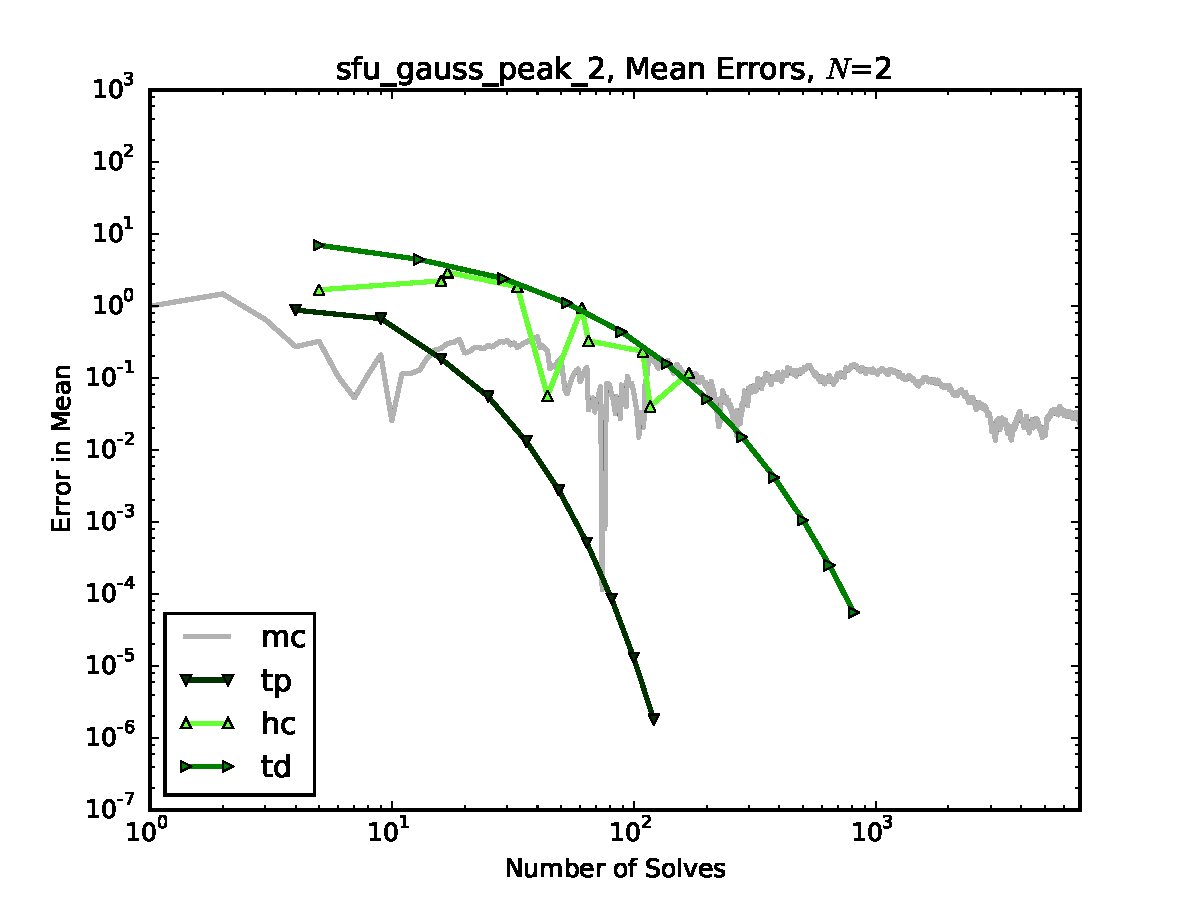
\includegraphics[width=0.7\linewidth]{sfu_gauss_peak_2_mean_errs.pdf}
  \caption{Gauss Peak, $N=2$, Mean Errors}
  \label{fig:gp2m}
\end{figure}
\begin{figure}[H]
  \centering
  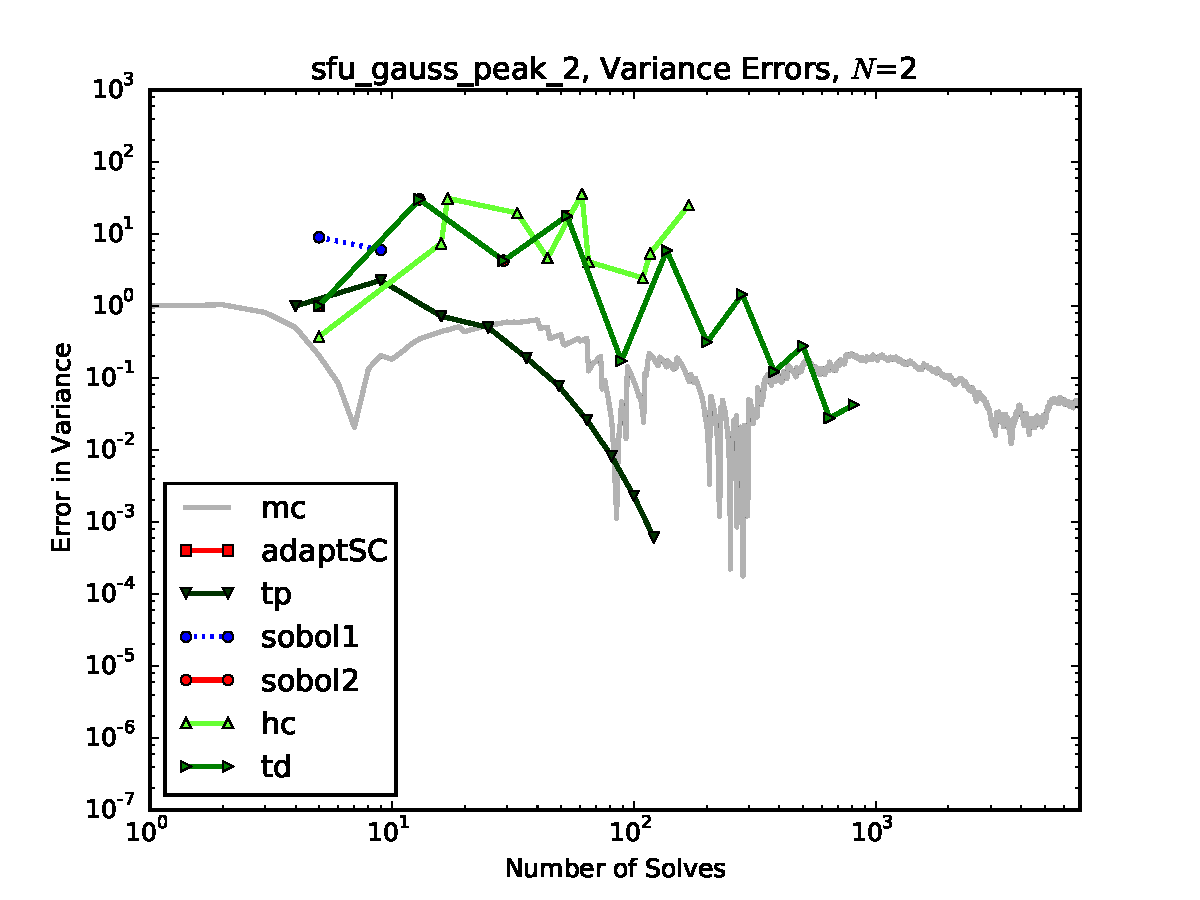
\includegraphics[width=0.7\linewidth]{sfu_gauss_peak_2_variance_errs.pdf}
  \caption{Gauss Peak, $N=2$, Variance Errors}
  \label{fig:gp2v}
\end{figure}

\begin{figure}[H]
  \centering
  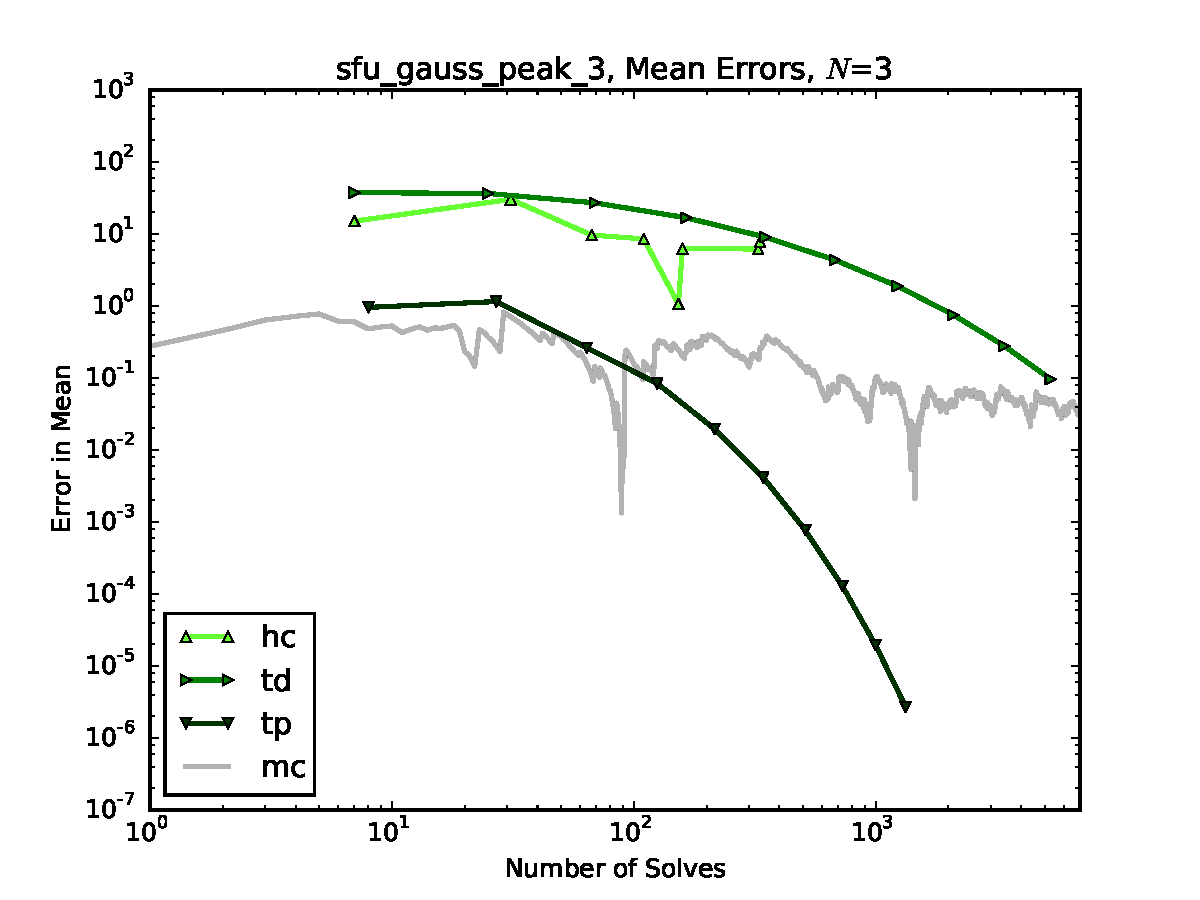
\includegraphics[width=0.7\linewidth]{sfu_gauss_peak_3_mean_errs.pdf}
  \caption{Gauss Peak, $N=3$, Mean Errors}
  \label{fig:gp3m}
\end{figure}
\begin{figure}[H]
  \centering
  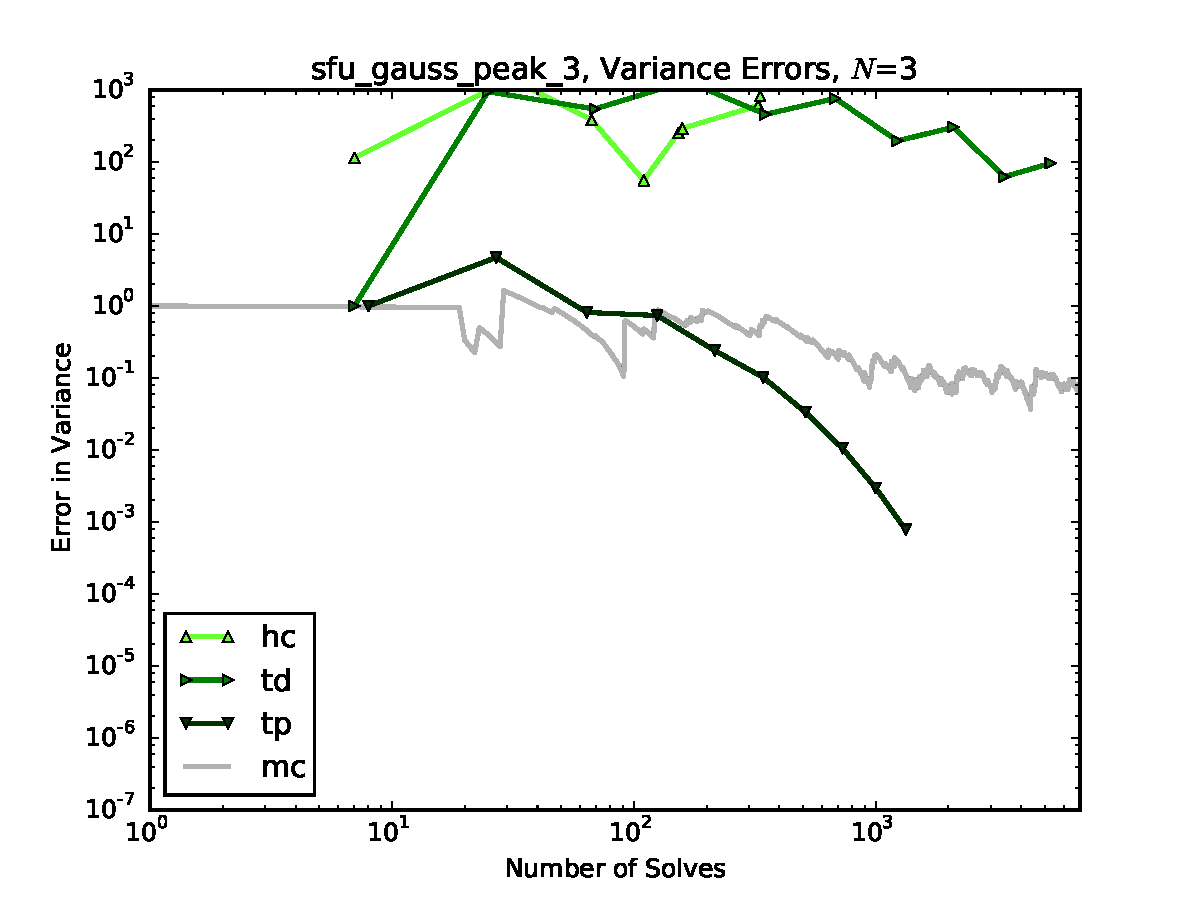
\includegraphics[width=0.7\linewidth]{sfu_gauss_peak_3_variance_errs.pdf}
  \caption{Gauss Peak, $N=3$, Variance Errors}
  \label{fig:gp3v}
\end{figure}

\section{Discussion}
From the figures, several trends are visibly apparent.\\

First, the Tensor Product collocation method converges exponentially for both mean and variance for both two-
and three-dimensional cases.\\

Second, the Total Degree collocation method appears to converge exponentially but in oscillations for both
mean and variance for the two-dimensional case, and the mean in the three-dimensional case; however, the
convergence is sufficiently slow that exponential convergence can't be guaranteed for the variance in the
three-dimensional case.\\

Third, Hyperbolic Cross collocation behaves erratically and quite poorly for this model.\\

Fourth, in all cases presented, it appears that Tensor Product both has a smaller magnitude of error and
converges more quickly than Total Degree.  This is somewhat unexpected, but since the form of the function
is tensor in polynomial expansion space (from Table \ref{tab:taylor}, perhaps this can be expected.
\end{document}
